\documentclass[tikz,border=3pt,10pt]{standalone}

\usepackage{fontspec}
\usepackage{unicode-math}
\usepackage{pgfplots}
\pgfplotsset{compat=1.18}

\setmainfont{STIXTwoText-Regular.otf}[
  Path=../../../../../../../assets/fonts/,
  BoldFont=STIXTwoText-Bold.otf,
  ItalicFont=STIXTwoText-Italic.otf,
  BoldItalicFont=STIXTwoText-BoldItalic.otf
]
\setmathfont{STIXTwoMath.otf}[
  Path=../../../../../../../assets/fonts/
]

% SỬA 1: bổ sung thư viện matrix vì hình có sử dụng \matrix.
\usetikzlibrary{backgrounds,matrix}
% ZO Math graph styles — VERSION 04 — 2026-07-27. % SỬA: cập nhật phiên bản.
% Global visual styles only; label positions belong to each graph source.
% Load \usetikzlibrary{backgrounds} before inputting this file.

\definecolor{zoWhite}{HTML}{FFFFFF}
\definecolor{zoPlotBackground}{HTML}{FFF9E9}
\definecolor{zoPlotBorder}{HTML}{DFD7CA}
\definecolor{zoBackground}{HTML}{FBFAF8}
\definecolor{zoGridMinor}{HTML}{F8F5F0}
\definecolor{zoGridMajor}{HTML}{DFD7CA}
\definecolor{zoAxis}{HTML}{554F48}
\definecolor{zoText}{HTML}{3E3A35}
\definecolor{zoTextStrong}{HTML}{25221F}
\definecolor{zoGraphMain}{HTML}{EF5350}
\definecolor{zoGraphStrong}{HTML}{997918} % SỬA: đồng bộ màu đường phụ với hình tham chiếu.
\definecolor{zoReference}{HTML}{997918}
\definecolor{zoHighlight}{HTML}{FFCA28}
\definecolor{zoHighlightLight}{HTML}{FFF4D4}
\definecolor{zoSuccess}{HTML}{1DE8B5}

\pgfplotsset{
  zo axis/.style={
    width=12cm,height=7.5cm,scale only axis, % SỬA: đồng bộ kích thước khung tham chiếu.
    axis equal image=false,enlargelimits=false,
    clip=true,clip mode=individual,
    axis lines=middle,grid=none,
    axis line style={draw=zoAxis,line width=0.8pt,<->},
    tick align=center,tickwidth=0.4mm,
    tick style={draw=zoAxis,line width=0.32pt},
    every axis x label/.append style={text=zoText,font=\normalsize}, % SỬA: chuẩn hóa nhãn trục x.
    every axis y label/.append style={text=zoText,font=\normalsize}, % SỬA: chuẩn hóa nhãn trục y.
    every tick label/.append style={text=zoText,font=\small}, % SỬA: chuẩn hóa chữ và số trên trục.
    every axis plot/.append style={line cap=round,line join=round}
  },
  zo grid/.style={
    major grid style={draw=zoGridMajor,line width=0.35pt},
    minor grid style={draw=zoGridMinor,line width=0.25pt}
  },
  zo graph main/.style={
    draw=zoGraphMain,line width=1.2pt,solid,no marks
  },
  zo graph secondary/.style={
    draw=zoGraphStrong,line width=0.9pt,solid,no marks
  },
  zo reference/.style={
    draw=zoReference,line width=0.6pt,dashed,no marks
  },
  zo asymptote/.style={
    draw=zoReference,line width=0.8pt,dashed,no marks
  },
  zo auxiliary line/.style={
    draw=zoAxis,line width=0.6pt,densely dashed,no marks
  },
  zo point closed/.style={
    only marks,
    mark=*,
    mark size=2.2pt,
    draw=zoGraphMain,
    fill=zoGraphMain
  },
  zo point open/.style={
    only marks,
    mark=*,
    mark size=2.2pt,
    draw=zoGraphMain,
    fill=zoPlotBackground,
    line width=0.8pt
  },
  zo point emphasized/.style={
    only marks,
    mark=*,
    mark size=2.8pt,
    draw=zoGraphStrong,
    fill=zoGraphStrong
  },
  zo point auxiliary/.style={
    only marks,
    mark=*,
    mark size=1.7pt,
    draw=zoReference,
    fill=zoReference
  }
}

\tikzset{
  zo graph field/.style={
    show background rectangle,
    inner frame sep=4mm,
    background rectangle/.style={
      fill=zoPlotBackground,
      draw=zoPlotBorder,
      line width=0.45pt,
      rounded corners=2mm
    }
  },
  zo axis label/.style={
    text=zoText,
    font=\normalsize
  }, % SỬA: thêm style chung cho nhãn trục.
  zo origin label/.style={
    text=zoText,
    font=\normalsize
  }, % SỬA: thêm style riêng cho nhãn gốc tọa độ O.
  zo graph label/.style={
    text=zoText,
    font=\small
  },
  zo point label/.style={
    text=zoText,
    font=\small
  },
  zo tick label/.style={
    text=zoText,
    font=\small
  }, % SỬA: thêm style cho các giá trị và ký hiệu đặt trên trục.
  zo reference label/.style={
    text=zoText,
    font=\small
  }, % SỬA: thêm style cho nhãn đường tham chiếu như y=x và y=-x.
  zo legend label/.style={
    text=zoText,
    font=\small
  }, % SỬA: thêm style cho công thức trong chú giải.
  zo auxiliary label/.style={
    text=zoText,
    font=\small
  } % SỬA: đổi từ \footnotesize sang \small.
}

% Hình 2 - phóng đại gần 0, phía x > 0.
% Đường cong được lấy mẫu đều theo u, với x = 1/u và y = sin(u).
% Nhãn số và chú giải đều là các \node độc lập.

\begin{document}
\begin{tikzpicture}[zo graph field]
  \begin{axis}[
    zo axis,
    width=12cm,
    height=7.5cm,
    xmin=-.015,
    xmax=0.345,
    ymin=-1.28,
    ymax=1.28,
    xtick={
      0.04897,0.05305,0.05787,0.06366,
      0.07074,0.07958,0.09095,0.10610,
      0.12732,0.15915,0.21221,0.31831
    },
    ytick={-1,1},
    xticklabels={},
    yticklabels={},
    xlabel={$x$},
    ylabel={},
    xlabel style={
      at={(axis description cs:1.025,0.5)},
      anchor=west,
      text=zoText,
      font=\normalsize
    },
    clip=false
  ]
    % u từ pi đến 8pi cho bảy nửa chu kỳ; không lấy mẫu đều theo x.
    \addplot[
      zo graph main,
      parametric,
      variable=\u,
      domain=pi:8*pi,
      samples=421
    ] ({1/\u},{sin(deg(\u))});

    % Các nghiệm z_n = 1/(n*pi) thuộc đồ thị.
    % Dấu x đặc nhận diện nghiệm mà không gợi nghĩa điểm bị loại.
    \addplot[
      only marks,
      mark=x,
      mark size=2.2pt,
      mark options={line width=0.9pt},
      draw=zoGraphMain
    ] coordinates {
      ({1/pi},0)
      ({1/(2*pi)},0)
      ({1/(3*pi)},0)
      ({1/(4*pi)},0)
      ({1/(5*pi)},0)
      ({1/(6*pi)},0)
    };

    % Các đường phụ chiếu cực trị xuống hoành độ c_n tương ứng.
    \draw[
      color=zoPlotBorder,
      line width=0.45pt,
      dashed
    ]
      (axis cs:{2/(3*pi)},0) -- (axis cs:{2/(3*pi)},-1);

    \draw[
      color=zoPlotBorder,
      line width=0.45pt,
      dashed
    ]
      (axis cs:{2/(5*pi)},0) -- (axis cs:{2/(5*pi)},1);

    \draw[
      color=zoPlotBorder,
      line width=0.45pt,
      dashed
    ]
      (axis cs:{2/(7*pi)},0) -- (axis cs:{2/(7*pi)},-1);

    \draw[
      color=zoPlotBorder,
      line width=0.45pt,
      dashed
    ]
      (axis cs:{2/(9*pi)},0) -- (axis cs:{2/(9*pi)},1);

    \draw[
      color=zoPlotBorder,
      line width=0.45pt,
      dashed
    ]
      (axis cs:{2/(11*pi)},0) -- (axis cs:{2/(11*pi)},-1);

    \draw[
      color=zoPlotBorder,
      line width=0.45pt,
      dashed
    ]
      (axis cs:{2/(13*pi)},0) -- (axis cs:{2/(13*pi)},1);

    \draw[
      color=zoPlotBorder,
      line width=0.45pt,
      dashed
    ]
      (axis cs:0,1) -- (axis cs:.345,1);

    \draw[
      color=zoPlotBorder,
      line width=0.45pt,
      dashed
    ]
      (axis cs:0,-1) -- (axis cs:.345,-1);

    % Sáu cực trị c_n = 2/((2n+1)*pi), n=1,...,6.
    % Các điểm được vẽ sau đường chiếu để dấu tròn luôn hiện rõ.
    \addplot[
      only marks,
      mark=*,
      mark size=1.75pt,
      draw=zoGraphMain,
      fill=zoGraphMain
    ] coordinates {
      ({2/(3*pi)},-1)
      ({2/(5*pi)},1)
      ({2/(7*pi)},-1)
      ({2/(9*pi)},1)
      ({2/(11*pi)},-1)
      ({2/(13*pi)},1)
    };

    % Nhãn trục: mỗi giá trị là một node độc lập.

    % SỬA 2: dùng style riêng cho gốc tọa độ để O có cỡ \normalsize.
    \node[
      zo origin label,
      anchor=north east,
      xshift=-4pt,
      yshift=-2pt
    ] at (axis cs:0,0) {$O$};

    \node[
      text=zoText,
      font=\small,
      anchor=north,
      xshift=0pt,
      yshift=-1pt
    ] at (axis cs:{1/(6*pi)},0) {$z_6$};

    \node[
      text=zoText,
      font=\small,
      anchor=north,
      xshift=0pt,
      yshift=-1pt
    ] at (axis cs:{1/(5*pi)},0) {$z_5$};

    \node[
      text=zoText,
      font=\small,
      anchor=north,
      xshift=0pt,
      yshift=-1pt
    ] at (axis cs:{1/(4*pi)},0) {$z_4$};

    \node[
      text=zoText,
      font=\small,
      anchor=north,
      xshift=0pt,
      yshift=-1pt
    ] at (axis cs:{1/(3*pi)},0) {$z_3$};

    \node[
      text=zoText,
      font=\small,
      anchor=north,
      xshift=0pt,
      yshift=-1pt
    ] at (axis cs:{1/(2*pi)},0) {$z_2$};

    \node[
      text=zoText,
      font=\small,
      anchor=north,
      xshift=0pt,
      yshift=-1pt
    ] at (axis cs:{1/pi},0) {$z_1$};

    % Dãy c_n đặt phía trên trục hoành.
    \node[
      text=zoText,
      font=\small,
      anchor=south,
      xshift=0pt,
      yshift=1pt
    ] at (axis cs:{2/(13*pi)},0) {$c_6$};

    \node[
      text=zoText,
      font=\small,
      anchor=south,
      xshift=0pt,
      yshift=1pt
    ] at (axis cs:{2/(11*pi)},0) {$c_5$};

    \node[
      text=zoText,
      font=\small,
      anchor=south,
      xshift=0pt,
      yshift=1pt
    ] at (axis cs:{2/(9*pi)},0) {$c_4$};

    \node[
      text=zoText,
      font=\small,
      anchor=south,
      xshift=0pt,
      yshift=1pt
    ] at (axis cs:{2/(7*pi)},0) {$c_3$};

    \node[
      text=zoText,
      font=\small,
      anchor=south,
      xshift=0pt,
      yshift=1pt
    ] at (axis cs:{2/(5*pi)},0) {$c_2$};

    \node[
      text=zoText,
      font=\small,
      anchor=south,
      xshift=0pt,
      yshift=1pt
    ] at (axis cs:{2/(3*pi)},0) {$c_1$};

    \node[
      text=zoText,
      font=\small,
      anchor=east,
      xshift=-2pt,
      yshift=0pt
    ] at (axis cs:0,-1) {$-1$};

    \node[
      text=zoText,
      font=\small,
      anchor=east,
      xshift=-2pt,
      yshift=0pt
    ] at (axis cs:0,1) {$1$};

    % Nhãn y neo trực tiếp trên đầu mũi tên của trục tung.
    \node[
      text=zoText,
      font=\normalsize,
      anchor=south,
      xshift=0pt,
      yshift=2pt
    ] at (axis cs:0,1.28) {$y$};

    \matrix[
      anchor=north east,
      at={(rel axis cs:1,1)},
      fill=zoWhite,
      draw=zoPlotBorder,
      line width=0.45pt,
      rounded corners=1mm,
      inner sep=5pt,
      row sep=3pt,
      column sep=5pt,
      ampersand replacement=\&,
      nodes={
        anchor=west,
        inner sep=0pt,
        outer sep=0pt
      }
    ] {
      \node[
        minimum width=5.5pt,
        minimum height=5.5pt
      ] {
        \tikz[baseline=-0.6ex]{
          \path[use as bounding box]
            (-2.75pt,-2.75pt) rectangle (2.75pt,2.75pt);
          \pgfsetstrokecolor{zoGraphMain}
          \pgfsetlinewidth{0.9pt}
          \pgfsetplotmarksize{2.2pt}
          \pgfuseplotmark{x}
        }
      }; \&
      \node[text=zoText,font=\small]
        {$z_n=\dfrac{1}{n\pi}$}; \\

      \node[
        minimum width=5.5pt,
        minimum height=5.5pt
      ] {
        \tikz[baseline=-0.6ex]{
          \path[use as bounding box]
            (-2.75pt,-2.75pt) rectangle (2.75pt,2.75pt);
          \pgfsetstrokecolor{zoGraphMain}
          \pgfsetfillcolor{zoGraphMain}
          \pgfsetplotmarksize{1.75pt}
          \pgfuseplotmark{*}
        }
      }; \&
      \node[text=zoText,font=\small]
        {$c_n=\dfrac{2}{(2n+1)\pi}$}; \\
    };

    % Dấu ba chấm chỉ phần tiếp tục dồn về 0, không thay cho dữ liệu vẽ.
    \node[
      text=zoText,
      font=\small,
      anchor=south,
      xshift=0pt,
      yshift=2pt
    ] at (axis cs:0.026,0) {$\ldots$};
  \end{axis}
\end{tikzpicture}
\end{document}